\documentclass[final,3p,12pt]{elsarticle}

% \documentclass[preprint,12pt]{elsarticle}

%% Use the option review to obtain double line spacing
%% \documentclass[authoryear,preprint,review,12pt]{elsarticle}

%% Use the options 1p,twocolumn; 3p; 3p,twocolumn; 5p; or 5p,twocolumn
%% for a journal layout:
% \documentclass[final,1p,times]{elsarticle}
%% \documentclass[final,1p,times,twocolumn]{elsarticle}
% \documentclass[final,3p,times]{elsarticle}
%% \documentclass[final,3p,times,twocolumn]{elsarticle}
% \documentclass[final,5p,times]{elsarticle}
%% \documentclass[final,5p,times,twocolumn]{elsarticle}
\usepackage[portuguese]{babel}

%% For including figures, graphicx.sty has been loaded in
%% elsarticle.cls. If you prefer to use the old commands
%% please give \usepackage{epsfig}

%% The amssymb package provides various useful mathematical symbols
\usepackage{amssymb}
\usepackage{amsmath}

\usepackage{multirow}

\usepackage{pgfplots}
\usepackage{placeins}
\usepackage{hyperref}

%=========== Gloabal Tikz settings
% \pgfplotsset{compat=newest}
% \usetikzlibrary{math}
% \pgfplotsset{
%     height = 10cm,
%     width = 10cm,
%     tick pos = left,
%     legend style={at={(0.98,0.30)}, anchor=east},
%     legend cell align=left,     
%     }
%  \pgfkeys{
%     /pgf/number format/.cd,
%     fixed,
%     precision = 1,
%     set thousands separator = {}
% }

%% The amsthm package provides extended theorem environments
%% \usepackage{amsthm}

%% The lineno packages adds line numbers. Start line numbering with
%% \begin{linenumbers}, end it with \end{linenumbers}. Or switch it on
%% for the whole article with \linenumbers.
%% \usepackage{lineno}

\usepackage{listings}
\usepackage{xcolor}

\definecolor{codegreen}{rgb}{0,0.6,0}
\definecolor{codegray}{rgb}{0.5,0.5,0.5}
\definecolor{codepurple}{rgb}{0.58,0,0.82}
\definecolor{backcolour}{rgb}{0.98,0.98,0.98}

\lstdefinestyle{mystyle}{
    backgroundcolor=\color{backcolour},   
    commentstyle=\color{codegreen},
    keywordstyle=\color{magenta},
    numberstyle=\tiny\color{codegray},
    stringstyle=\color{codepurple},
    basicstyle=\ttfamily\footnotesize,
    breakatwhitespace=false,         
    breaklines=true,                 
    captionpos=b,                    
    keepspaces=true,                 
    numbers=left,                    
    numbersep=5pt,                  
    showspaces=false,                
    showstringspaces=false,
    showtabs=false,                  
    tabsize=2
}

\lstset{style=mystyle}

% \journal{Nuclear Physics B}

\begin{document}

\begin{frontmatter}

%% Title, authors and addresses

%% use the tnoteref command within \title for footnotes;
%% use the tnotetext command for theassociated footnote;
%% use the fnref command within \author or \address for footnotes;
%% use the fntext command for theassociated footnote;
%% use the corref command within \author for corresponding author footnotes;
%% use the cortext command for theassociated footnote;
%% use the ead command for the email address,
%% and the form \ead[url] for the home page:
%% \title{Title\tnoteref{label1}}
%% \tnotetext[label1]{}
%% \author{Name\corref{cor1}\fnref{label2}}
%% \ead{email address}
%% \ead[url]{home page}
%% \fntext[label2]{}
%% \cortext[cor1]{}
%% \affiliation{organization={},
%%             addressline={},
%%             city={},
%%             postcode={},
%%             state={},
%%             country={}}
%% \fntext[label3]{}

\title{Aplicação do Método de Newton-Raphson para Resolver o Cálculo Inverso do Método da Mínima Curvatura\tnoteref{label_title}}
\tnotetext[label_title]{Relatório número 2 como parte dos requisitos da disciplina IM253: Métodos Numéricos para Fenômenos de Transporte.}

%% use optional labels to link authors explicitly to addresses:
%% \author[label1,label2]{}
%% \affiliation[label1]{organization={},
%%             addressline={},
%%             city={},
%%             postcode={},
%%             state={},
%%             country={}}
%%
%% \affiliation[label2]{organization={},
%%             addressline={},
%%             city={},
%%             postcode={},
%%             state={},
%%             country={}}

\author{Tiago C. A. Amorim\fnref{label_author}}
\tnotetext[label_author]{Atualmente cursando doutorado no Departamento de Engenharia de Petróleo da Faculdade de Engenharia Mecânica da UNICAMP (Campinas/SP, Brasil).}
\ead{t100675@dac.unicamp.br}
\affiliation[Tiago C. A. Amorim]{organization={Petrobras},%Department and Organization
addressline={Av. Henrique Valadares, 28}, 
city={Rio de Janeiro},
postcode={20231-030}, 
state={RJ},
country={Brasil}}

\begin{abstract}

\end{abstract}


%%Graphical abstract
% \begin{graphicalabstract}
%\includegraphics{grabs}
% \end{graphicalabstract}

%%Research highlights
% \begin{highlights}
% \item Research highlight 1
% \item Research highlight 2
% \end{highlights}

\begin{keyword}
    Método da Mínima Curvatura \sep Método de Newton-Raphson
%% keywords here, in the form: keyword \sep keyword

%% PACS codes here, in the form: \PACS code \sep code

%% MSC codes here, in the form: \MSC code \sep code
%% or \MSC[2008] code \sep code (2000 is the default)

\end{keyword}

\end{frontmatter}

%% \linenumbers

%% main text
\section{Introdução}

O Método da Mínima Curvatura possibilita o cálculo de cooordenadas cartesianas ($\Delta$N, $\Delta$E, $\Delta$V) a partir de parâmetros perfuração ($\Delta$S, $\theta$, $\phi$) assumindo que a trajetória de um poço direcional pode ser descrita como uma série de arcos \cite{10.2118/84246-MS}. Não existe formulação direta para o cálculo inverso, isto é, dos parâmetros de perfuração em função das coordenadas cartesianas.

No primeiro relatório desta série \cite{relatoriobisseccao} foi apresentada uma proposta de metodologia para cálculo dos parâmetros de perfuração a partir das coordenadas cartesianas de pontos ao longo da geometria do poço. O algoritmo proposto tem formulação implícita e foi organizado como um problema do tipo $g(x)=x$. O problema foi resolvido com o Método da Bissecção, encontrando bons resultados.

Neste segundo relatório é aplicado o método de Newton-Raphson de para resolver o mesmo problema.

\section{Metodologia}

\subsection{Derivada do Algoritmo Proposto}

A seguir são apresentadas as fórmulas que foram do algoritmo proposto para cálculo de parâmetros de perfuração em função de coordenadas cartesianas \cite{relatoriobisseccao}. O algoritmo assume que para calcular os parâmtros de perfuração entre dois pontos quaisquer são conhecidos os parâmetros de perfuração do ponto inicial\footnote{Para o primeiro ponto da trajetória é assumido um poço na vertical: $\theta=0$, $\phi=0$.} ($\theta_1$, $\phi_1$) e as distâncias cartesianas entre os pontos ($\Delta$N,$\Delta$E, $\Delta$V). O objetivo é calcular $\theta_2$, $\phi_2$ e $\Delta S$:

\begin{equation} \label{eq:costheta2}
    \cos \theta_2 = 2 \frac{\Delta V}{\Delta S f(\alpha)} - \cos \theta_1
\end{equation}
\begin{equation} \label{eq:sinphi2}
    \sin \phi_2 = \frac{-\Delta N \Delta \Psi}{\Delta H^2} \left( \frac{\sin \theta_1}{\sin \theta_2} \right) + \frac{\Delta E}{\Delta H^2} \sqrt{\Delta H^2 - \Delta \Psi^2 \left( \frac{\sin \theta_1}{\sin \theta_2} \right)^2} 
\end{equation}
\begin{equation} \label{eq:cosphi2}
    \cos \phi_2 = \frac{\Delta E \Delta \Psi}{\Delta H^2} \left( \frac{\sin \theta_1}{\sin \theta_2} \right) + \frac{\Delta N}{\Delta H^2} \sqrt{\frac{1}{\Delta H^2} - \Delta \Psi^2 \left( \frac{\sin \theta_1}{\sin \theta_2} \right)^2} 
\end{equation}
\begin{align*}
    \intertext{onde}
    \Delta \Psi &= \Delta N \sin \phi_1 - \Delta E \cos \phi_1 \\
    \Delta H^2 &= \Delta N^2 + \Delta E^2
\end{align*}
\begin{equation} \label{eq:DeltaSfa}
    \Delta S f(\alpha) = 2 \sqrt{\frac{\Delta N^2 + \Delta E^2 + \Delta V^2}{A^2+B^2+C^2}}
\end{equation}
\begin{align*}
    \intertext{onde}
    A &= \sin \theta_1 \cos \phi_1 + \sin \theta_2 \cos \phi_2 \\
    B &= \sin \theta_1 \sin \phi_1 + \sin \theta_2 \sin \phi_2 \\
    C &= \cos \theta_1 + \cos \theta_2
\end{align*}

Com as equações propostas é possível construir uma função do tipo $g(x)=x$:

\begin{enumerate}
    \item Assumir um valor inicial de $\Delta S f(\alpha)$.
    \item Calcular $\cos \theta_2$ com a equação \ref{eq:costheta2}.
    \item Calcular $\sin \phi_2$ com a equação \ref{eq:sinphi2}.
    \item Calcular $\cos \phi_2$ com a equação \ref{eq:cosphi2}.
    \item Calcular $\Delta S f(\alpha)$ com a equação \ref{eq:DeltaSfa}.
\end{enumerate}

Em \cite{relatoriobisseccao} são discutidos detalhes adicionais sobre a implementação deste algoritmo.

Para utilizar o método de Newton-Raphson para resolver o problema proposto, será preciso encontrar a derivada da função com relação a $x$ de $f(x) = g(x) - x$. Para facilitar a leitura, $\Delta S f(\alpha)$ é substituído por $x$ na equação \ref{eq:DeltaSfa}, e então é definida a função $f(x)$\footnote{Os termos que dependem de $\Delta S$ serão explicitados usando $(x)$.}:

\begin{equation} \label{eq:fx}
    f(x) = 2 \sqrt{\frac{\Delta N^2 + \Delta E^2 + \Delta V^2}{A(x)^2+B(x)^2+C(x)^2}} - x
\end{equation}

\begin{align*}
    \intertext{onde}
    A(x) &= \sin \theta_1 \cos \phi_1 + \sin \theta_2(x) \cos \phi_2(x) \\
    B(x) &= \sin \theta_1 \sin \phi_1 + \sin \theta_2(x) \sin \phi_2(x) \\
    C(x) &= \cos \theta_1 + \cos \theta_2(x)
\end{align*}

Derivando $f(x)$:

\begin{equation} \label{eq:fxprime}
    f(x)^{\prime} = - \frac{2}{\Delta S^2} \left( \frac{ \Delta N^2 + \Delta E^2 + \Delta V^2}{A(x)^2+B(x)^2+C(x)^2} \right) ^{3/2} [A(x)A(x)^{\prime}+B(x)B(x)^{\prime}+C(x)C(x)^{\prime}] - 1
\end{equation}

\begin{align*}
    \intertext{onde}
    A(x)^{\prime} &= \sin \theta_2(x)^{\prime} \cos \phi_2(x) + \sin \theta_2(x) \cos \phi_2(x)^{\prime} \\
    B(x)^{\prime} &= \sin \theta_2(x)^{\prime} \sin \phi_2(x) + \sin \theta_2(x) \sin \phi_2(x)^{\prime} \\
    C(x)^{\prime} &= \cos \theta_2(x)^{\prime}
\end{align*}

Os demais termos das equações são obtidos derivando as equações \ref{eq:costheta2}, \ref{eq:sinphi2} e \ref{eq:cosphi2}:

\begin{equation} \label{eq:costheta2prime}
    \cos \theta_2(x)^{\prime} = - \frac{2 \Delta V}{x^2} 
\end{equation}

\begin{equation} \label{eq:sinphi2prime}
    \sin \phi_2(x)^{\prime} = \frac{\cfrac{\Delta \Psi \sin \theta_1}{\sin \theta_2(x)}}{\Delta H^2} \left( \Delta N + \Delta E \frac{\cfrac{\Delta \Psi \sin \theta_1}{\sin \theta_2(x)} }{\sqrt{\Delta H^2 - \left( \cfrac{\Delta \Psi \sin \theta_1}{\sin \theta_2(x)} \right)^2}} \right) \frac{\sin \theta_2(x)^{\prime}}{\sin \theta_2(x)} 
\end{equation}
\begin{equation} \label{eq:cosphi2prime}
    \cos \phi_2(x)^{\prime} = \frac{\cfrac{\Delta \Psi \sin \theta_1}{\sin \theta_2(x)}}{\Delta H^2} \left( \Delta E - \Delta N \frac{\cfrac{\Delta \Psi \sin \theta_1}{\sin \theta_2(x)} }{\sqrt{\Delta H^2 - \left( \cfrac{\Delta \Psi \sin \theta_1}{\sin \theta_2(x)} \right)^2}} \right) \frac{\sin \theta_2(x)^{\prime}}{\sin \theta_2(x)} 
\end{equation}

onde $\Delta \Psi$ e $\Delta H^2$ seguem as mesmas definições das equações \ref{eq:sinphi2} e \ref{eq:cosphi2}.

A definição de $\sin \theta_2(x)^{\prime}$ pode ser desenvolvida a partir de $\cos^2 \theta_2(x) + \sin^2 \theta_2(x) = 1$:
\begin{equation} \label{eq:sintheta2prime}
    \sin \theta_2(x)^{\prime} = - \frac{\frac{2 \Delta V}{x}(\cos \theta_1 - \frac{2 \Delta V}{x})}{x \sqrt{1-\left(\cos \theta_1 - \frac{2 \Delta V}{x} \right)^2}}
\end{equation}

    \subsection{Método de Newton-Raphson}
    
    O código desenvolvido foi baseado no pseudo-código de \cite{burden2016analise}. O Método de Newton-Raphson faz uso da derivada da função de interesse. O método precisa apenas de um ponto inicial, e converge mais rápido que o Método da Bissecção, mas não tem garantia de encontrar uma raiz. 

    De modo simplificado o Método de Newton-Raphson pode ser descrito como:
    
    \begin{enumerate}
        \item Definir $x_0$.
        \item Iniciar contagem de iterações com $i=0$.
        \item Calcular $f(x_i)$ e $f(x_i)^{\prime}$.
        \item Calcular $x_{i+1} = x_i - \frac{f(x_i)}{f(x_i)^{\prime}}$.
        \item Incrementar a contagem de iterações: $i=i+1$.
        \item Se não atingiu critério de convergência, retornar para passo 3.
        \item Retornar $x_{i+1}.$.
    \end{enumerate}
    
    Foram adicionados critérios adicionais ao algoritmo para controlar o processo iterativo:

    \begin{itemize}
        \item Foram implementados dois métodos de cálculo do critério de convergência\footnote{Ver descrição em \cite{relatoriobisseccao}.}: \emph{Direto} e \emph{Relativo}.
        \item É feito um término prematuro do processo iterativo caso algum $|f(x)| < \epsilon$. O valor padrão de $\epsilon$ é $10^{-7}$ (variável \verb|epsilon| no código). Este teste também é feito antes de entrar no \emph{loop}.
        \item A cada iteração é verificado se a derivada da função está muito próxima de zero: $|f(x)^{\prime}| < \epsilon$. Em caso positivo é gerada uma mensagem e é encerrado o \emph{loop}.
        \item Como o método não garante convergência, ao longo das iterações é guardado o melhor resultado ($x$ tal que $|f(x)|$ seja mínimo). Este é o resultado que é retornado.
    \end{itemize}
    
    \section{Resultados}
    
    Para facilitar a análise da qualidade do código desenvolvido, foram criadas funções que realizam diversos testes onde a resposta exata é conhecida:

    \begin{description}
        \item[tests\textunderscore newton\textunderscore raphson()] Testa o Método de Newton-Raphson em diferentes funções: linear, quadrática, exponencial e trigonométrica. Também foram apicados casos específicos para o algoritmo tratar: raiz no ponto inicial, ponto inicial muito próximo da raiz, ponto inicial em um ponto de mínimo da função (derivada nula), uso de critério de convergência relativo, função com derivada nula na raiz, função com vários mínimos e máximos locais.
        
        \item[tests\textunderscore minimum\textunderscore curvature()] Testa as funções implementadas para cálculo de coordenadas cartesianas em função de parâmetros de perfuração (cálculo direto), e de parâmetros de perfuração em função de coordenadas cartesianas (cálculo iterativo).
    \end{description}

    A implementação do Método de Newton-Raphson teve uma alteração adicional em função dos resultados dos testes realizados. Nas fórmulas do problema proposto fica evidente que a variável principal ($\Delta S f(\alpha)$) não pode ter um valor qualquer. Para evitar simplesmente parar o processo iterativo quando o próximo ponto é menor que o limite inferior, foi implementada uma verificação adicional no método: caso o novo valor de $x$ estiver fora dos limites pré-estabelecidos, usará o valor do limite que foi violado. Desta forma é dada uma \emph{chance} para o processo iterativo conseguir convergir para uma resposta melhor. Para os cálculos de parâmetros de perfuração foi utilizado um limite inferior de $\Delta S f(\alpha)$ igual ao discutido em \cite{relatoriobisseccao}.

    Como esperado, o Método de Newton-Raphson se mostrou mais rápido que o Método da Bissecção (Tabela \ref{table:iteracoes}). O único teste em que o Método da Bissecção teve uma convergência melhor foi na função exponencial: $\exp^{x^2-4}-1$. Enquanto o Método da Bisseção tem convergência linear, o Método de Newton-Raphson teve convergência aproximadamente quadrática (). 

    \begin{table}[h] 
        \centering
        \caption{Comparação entre o número de iterações necessários para um mesmo critério de convergência usando os Métodos da Bissecção e Newton-Raphson.}
        \begin{tabular}{ l c c c c c c }
            \multirow{2}{*}{Função} & \multirow{2}{*}{Raiz} & \multicolumn{3}{c}{Bissecção} & \multicolumn{2}{c}{Newton-Raphson} \\
              &  & $x_a$ & $x_b$ & Iter. & $x_0$ & Iter. \\ 
            \hline
            Linear & 0.3 & 0. & 2. &  11 & 0. & 1\\
            Quadrática & -0.1 & -0.25 & 1. & 11 & 0.25 & 4  \\
            Exponencial  & 2. & 0. & 10. & 14 & 5. & 25 \\
            Trigonométrica & $3\pi/4$ & 0. & 5. & 13 & 3. & 3  \\
            1/4 círculo horizontal & 20 & 14.1421 & 120.417 & 17 & 14.4743 & 1 \\
            Seção 2 do poço em S & 131.652 & 130.526 & 1111.4 & 20 & 133.592 & 11 \\
            Poço 3D & 10.3144 & 9.84918 & 83.8634 & 17 & 10.0805 & 4 \\
        \end{tabular}
        \label{table:iteracoes}
    \end{table}
    
    Na aplicação do Método de Newton com o algoritmo desenvolvido para cálculo de parâmetros de perfuração os resultados foram muito bons. Nenhum dos testes teve problemas de convergência, e convergiram com um número de iterações menor que o do Método da Bissecção ().

    Para algumas funções o Método de Newton-Raphson se mostrou instável, ficando muito dependente do ponto inicial para conseguir convergir. A função $\cos x + \sin x$ tem muitas raízes, e o resultado do Método de Newton-Raphson se mostrou muito dependente do ponto inicial. Para conseguir encontrar a raiz de uma determinada região foi preciso definir um ponto inicial \emph{bem próximo} da raiz. Já a função $3x + x^2 \sin^2 \frac{x\pi}{10}$ mostrou muita instabilidade, em muitos casos não conseguindo convergir.

    Para o problema proposto foram testados alguns valores distintos de ponto inicial (Tabela ).
    
    \section{Conclusão}
    
    O algoritmo proposto para o cálculo de parâmetros de perfuração em função das coordenadas cartesianas de pontos ao longo do se mostrou eficaz. Foram feitos ajustes ao código implementado de forma a evitar o uso de funções trigonométricas ao longo do processo iterativo.
    O Método da Bisseção se mostrou adequado para uso com o algoritmo proposto. As funções propostas não são válidas para quaisquer valores de entrada, e a delimitação de uma região de busca foi importante para garantir a convergência do problema.

    % \label{}
    
%% The Appendices part is started with the command \appendix;
%% appendix sections are then done as normal sections
%% \appendix

%% \section{}
%% \label{}

%% If you have bibdatabase file and want bibtex to generate the
%% bibitems, please use
%%

\bibliographystyle{elsarticle-num} 
\bibliography{refs}

%% else use the following coding to input the bibitems directly in the
%% TeX file.

% \begin{thebibliography}{00}

%% \bibitem{label}
%% Text of bibliographic item

% \bibitem{}

% \end{thebibliography}

\newpage

\appendix

% \FloatBarrier
% \section{Gráficos Diagnóstico}

% \subsection{Erro ao Longo da Iterações}

% A figura abaixo apresenta a evolução do erro, com relação à resposta exata, ao longo do processo iterativo de diferentes funções, utilizando o Método da Bissecção. São apresentadas duas retas tracejadas onde a razão entre os erros de iterações sucessivas é 0.5, que é o que se espera do Método da Bissecção após um número considerável de iterações. Observa-se que os resultados numéricos não seguem exatamente uma linha reta, mas têm aproximadamente a mesma inclinação das retas tracejadas.

% \begin{figure}[hbt!] 
%     \label{fig:Erro}
%     \centering
%     \begin{tikzpicture}
%         \begin{axis}[
%             height = 10cm, % standard 10cm
%             width = 0.8\textwidth, %15cm,  % standard 10cm
%             % xmode=log,
%             ymode=log,
%             grid=both,
%             % ymin=1e-12,
%             % ymax=1e0,
%             xlabel = {Iterações},
%             ylabel = {$\varepsilon_i = |P_i - P|$},
%             legend style={at={(0.99,0.80)}, anchor=east},
%             ]
%             \addplot[color=black, solid, mark=*] table [x=Iteration, y =Linear] {IterationError.txt};
%             \addplot[color=blue, solid, mark=*] table [x=Iteration, y =Quadratic] {IterationError.txt};
%             \addplot[color=green, solid, mark=*] table [x=Iteration, y =Exponential] {IterationError.txt};
%             \addplot[color=red, solid, mark=*] table [x=Iteration, y =Trigonometric] {IterationError.txt};
%             \addplot[color=purple, solid, mark=*] table [x=Iteration, y =3Dwell] {IterationError.txt};
%             \addplot[color=black, dashed] table [x=Iteration, y =TX05A] {IterationError.txt};
%             \addplot[color=black, dashed] table [x=Iteration, y =TX05B] {IterationError.txt};
%             \legend{Linear, Quadrática, Exponencial, Trigonométrica, Poço 3D};
%         \end{axis}
        
%     \end{tikzpicture}
%     \caption{Evolução do erro do Método da Bissecção com diferentes funções (linhas tracejadas representam $\varepsilon_{i+1} / \varepsilon_i = 0.5$).}
% \end{figure}

% \newpage
% \FloatBarrier
% \subsection{Erro em Função do Limite de Convergência}

% A figura a seguir mostra os erros (com relação ao valor exato) nas estimativas de diferentes parâmetros de perfuração. O algoritmo proposto foi aplicado a um trecho de poço com mudança em inclinação e direção, utilizando diferentes valores de limite de convergência ($c_{lim}$).

% \begin{figure}[hbt!]
%     \label{fig:convergencia}
%     \centering
%     \begin{tikzpicture}
%         \begin{axis}[
%             height = 10cm, % standard 10cm
%             width = 0.8\textwidth, %15cm,  % standard 10cm
%             xmode=log,
%             ymode=log,
%             grid=both,
%             ymin=1e-12,
%             ymax=1e0,
%             xlabel = {$c_{lim}$},
%             ylabel = {Erro},
%             legend style={at={(0.25,0.55)}, anchor=east},
%             ]
%             \addplot[color=black, solid, mark=*] table [x=Convergence, y = DeltaSfa] {ConvergenceErrors.txt};
%             \addplot[color=purple, solid, mark=*] table [x=Convergence, y = DeltaS] {ConvergenceErrors.txt};
%             \addplot[color=blue, solid, mark=*] table [x=Convergence, y = theta2] {ConvergenceErrors.txt};
%             \addplot[color=green, solid, mark=*] table [x=Convergence, y = phi2] {ConvergenceErrors.txt};
%             \legend{$\Delta S f(\alpha)$, $\Delta S$, $\theta_2$, $\phi_2$};
%         \end{axis}
        
%         \begin{axis}[
%             height = 10cm, % standard 10cm
%             xmode=log,
%             width = 0.8\textwidth, %15cm,  % standard 10cm
%             axis y line=right,
%             ylabel={Iterações até Convergência},
%             ymin=0,
%             ymax=50,
%             % yticklabel style={red},
%             legend style={at={(0.98,0.10)}, anchor=east},
%             ]
%             \addplot[color=red, solid, mark=*] table [x=Convergence, y = Iterations] {ConvergenceErrors.txt};
%             \legend{Iterações}
%         \end{axis}

%     \end{tikzpicture}
%     \caption{Erro das variáveis de interesse em função do limite de convergência utilizado.}
% \end{figure}

% \newpage
% \FloatBarrier
% \section{Esquema do Poço em S}

% Um dos exemplos testados com o algoritmo proposto para calcular parâmetros de perfuração em função de coordenadas cartesianas é um poço em S. Uma representação esquemática da trajetória do poço (sem escala) é apresentada abaixo.

% \begin{figure}[hbt!]
%     \label{fig:pocoS}
%     \centering
%     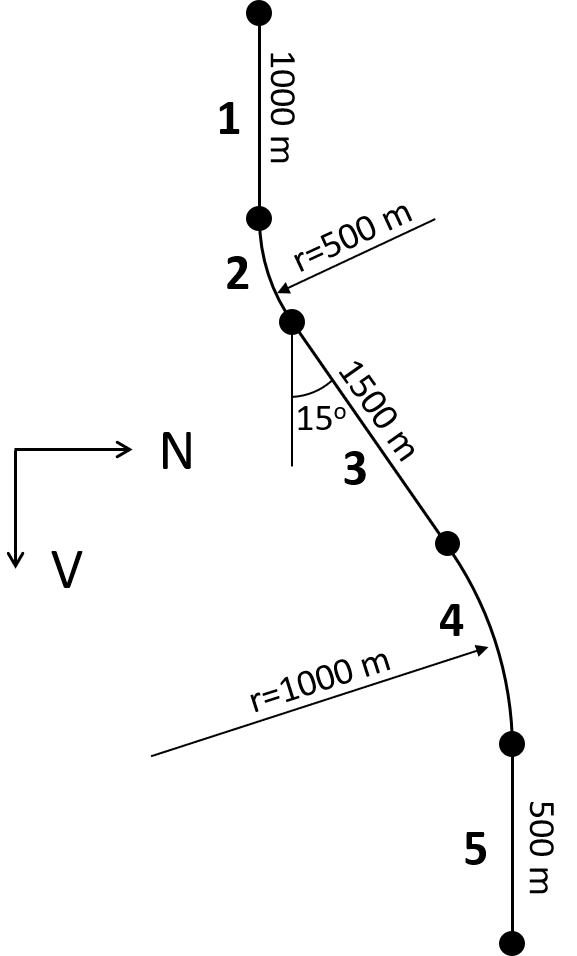
\includegraphics[width=0.4\textwidth]{EsquemaPoco}
%     \caption{Esquema do poço em 'S' descrito nos testes de tests\textunderscore minimum\textunderscore curvature().}
% \end{figure}

\newpage
\FloatBarrier
\section{Código em C}

O código de ambos métodos foi implementado em um único arquivo. O código é apresentado em duas partes neste documento para facilitar a leitura. O código pode ser encontrado em \href{https://github.com/TiagoCAAmorim/numerical-methods}{https://github.com/TiagoCAAmorim/numerical-methods}.

\subsection{Método de Newton-Raphson}
% \lstinputlisting[language=C, linerange={1-276}]{./01_bissection.c}

\subsection{Método da Mínima Curvatura}
% \lstinputlisting[language=C, linerange={279-999}]{./01_bissection.c}

\end{document}
\endinput